\documentclass[40pt,a4paper,UTF8]{ctexart}
\usepackage{amsmath}
\usepackage{graphicx}

\usepackage{float}

%输入带圈数字  eg:\textcircled{1}
\usepackage{fontspec,xunicode-addon}

%代码显示的包
\usepackage{listings}
\usepackage{xcolor}

%打出空心字母
\usepackage{amsfonts,amssymb}

%整体加粗
\usepackage{bm}

%公式按照章节标号
\numberwithin{equation}{section}

%长等号
\usepackage{extpfeil}

%注释用
\usepackage{comment}
%----------------------------------------------
%配置代码显示格式-掌握minted之前的替代品
%----------------------------------------------
\definecolor{codegreen}{rgb}{0,0.6,0}
\definecolor{codegray}{rgb}{0.5,0.5,0.5}
\definecolor{codepurple}{rgb}{0.58,0,0.82}
\definecolor{backcolour}{rgb}{0.95,0.95,0.92}

\lstdefinestyle{mystyle}{
	backgroundcolor=\color{backcolour},   
	commentstyle=\color{codegreen},
	keywordstyle=\color{magenta},
	numberstyle=\tiny\color{codegray},
	stringstyle=\color{codepurple},
	basicstyle=\ttfamily\footnotesize,
	breakatwhitespace=false,         
	breaklines=true,                 
	captionpos=b,                    
	keepspaces=true,                 
	numbers=left,                    
	numbersep=5pt,                  
	showspaces=false,                
	showstringspaces=false,
	showtabs=false,                  
	tabsize=2
}

\lstset{style=mystyle}



%-----------------------------------------------------------------------------------

\title{第五章作业}
\author{Student name: Francisrk}
\date{Due date: March 6th, 2022}

\begin{document}

\maketitle   %控制序列,能将在导言区中定义的标题、作者、日期按照预定的格式展现出来。

\section{第1题}
\paragraph{}
已阅。
\paragraph{}


\section{第2题}
\paragraph{}

\subsection{ORB提取}
提取方向的思想是以每个FAST角点为中心取16*16的方形像素区域,一半为8,那么为了保证能取到,需要对边界进行处理,对于x<8或y<8或(x>列数-8)或(y>行数-8)的点都是不能取patch的,然后计算$m_{10}$和$m_{01}$,使用std::atan2计算出弧度,再$*\frac{180}{\pi}$即得角度,代码如下所示:
\begin{lstlisting}[language=C++, caption=computeORB.cpp]
void computeAngle(const cv::Mat &image, vector<cv::KeyPoint> &keypoints) {
    int half_patch_size = 8;
//  int half_boundry = 16;
    int bad_points =0;   //角点中不能计算角度的点
    for (auto &kp : keypoints) {
        // START YOUR CODE HERE (~7 lines)
        int u=kp.pt.x, v = kp.pt.y;
        if(u>=half_patch_size && v>=half_patch_size && u+half_patch_size<=image.cols && v+half_patch_size<=image.rows)
        {
            float m01=0, m10=0;
            for(int i=u-half_patch_size; i < u + half_patch_size; ++i)  //x方向遍历16个点(右)
                for(int j=v-half_patch_size; j < v + half_patch_size; ++j)  //y方向遍历16个点(下)
                {
                    m10 +=i * image.at<uchar>(j, i);
                    m01 +=j * image.at<uchar>(j, i);
                }
            //计算角度(弧度制)并转换为角度
            kp.angle = (float)std::atan(m01/m10) * 180/pi ;  //或者std::atan2(m01, m10)*180/pi;
        }
        // END YOUR CODE HERE
    }
    return;
}

\end{lstlisting}


\begin{figure}[H]
\centering
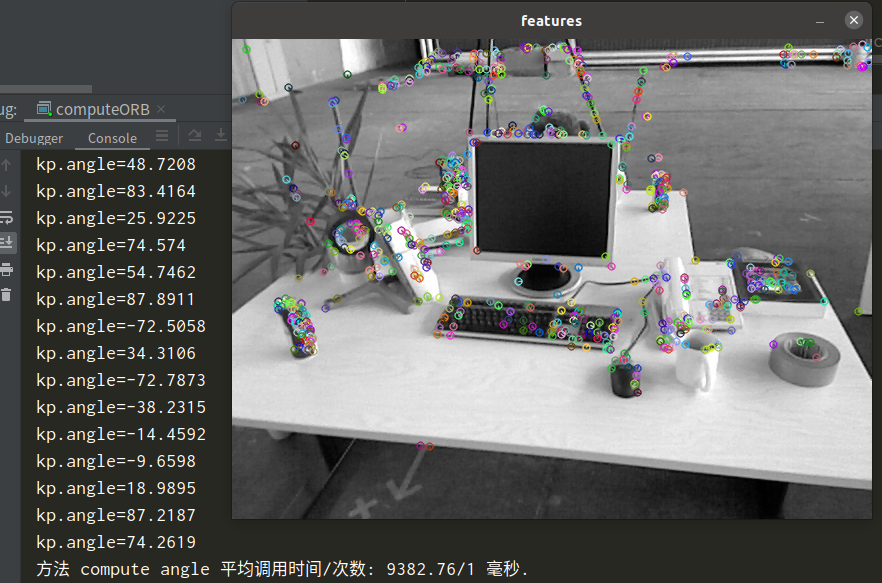
\includegraphics[width=4.8in]{ch5_2_1.png} {图2.1 角度计算和ORB特征显示}
\end{figure}

\subsection{ORB描述}
核心任务有两个:

STEP1:检查是否越界,如果越界则认为不是好角点,描述子为空;

STEP2:若不越界,则根据pattern来采集点,结合特征点的方向角theta来旋转点p,q->p',q',计算p',q'的坐标,同时也要判断坐标是否越界,若越界,此次描述子清零,跳出循环;

STEP3:若不越界,比较大小,结果作为该位描述子的结果(0 or 1)。

代码如Listing2所示,运行结果如图2.2所示。

\begin{lstlisting}[language=C++, caption=computeORB.cpp]
void computeORBDesc(const cv::Mat &image, vector<cv::KeyPoint> &keypoints, vector<DescType> &desc)
{
    int half_patch_size = 8, bad_points = 0;
    for (auto &kp : keypoints)
    {
        int u = kp.pt.x, v = kp.pt.y;
        DescType d(256, false);   //256位描述子
        //STEP1:检查是否越界
        if(u>=half_patch_size && v>=half_patch_size && u+half_patch_size<=image.cols && v+half_patch_size<=image.rows)
        {
            //STEP2:若不越界,则根据pattern来采集点,结合特征点的方向角theta来旋转点p,q->p',q',计算p',q'的坐标,并比较大小,结果作为该位描述子的结果(0 or 1)
            for (int i = 0; i < 256; i++)
            {
                // START YOUR CODE HERE (~7 lines)
                //寻找取点pattern的下标
                cv::Point2f p(ORB_pattern[i * 4], ORB_pattern[i * 4 + 1]);
                cv::Point2f q(ORB_pattern[i * 4 + 2], ORB_pattern[i * 4 + 3]);

                //使用sin,cos, 角度转换为弧度 *pi/180
                double theta = kp.angle * pi / 180;
                double cos_theta = cos(theta) , sin_theta = sin(theta);

                int u_p_ = (int)(cos_theta * p.x - sin_theta * p.y) + u;
                int v_p_ = (int)(sin_theta * p.x + cos_theta * p.y) + v;
                int u_q_ = (int)(cos_theta * q.x - sin_theta * q.y) + u;
                int v_q_ = (int)(sin_theta * q.x + cos_theta * q.y) + v;
                //判断根据关键点得到的经过旋转的p、q是否出界,若出界,则该描述子清空作废
                if(u_p_<0 || v_p_<0 || u_p_ >image.cols || v_p_ > image.rows || u_q_<0 || v_q_<0 || u_q_ >image.cols || v_q_ > image.rows)
                {
                    d = {};
                    break;  //跳出描述子循环
                }
                d[i] = image.at<uchar>(v_p_, u_p_) > image.at<uchar>(v_q_, u_q_) ? false : true;  //前者大取false,后者大取true,vector随机访问器,不够快,但是掌握算法是关键
            }
        }
        //越界则不使用
        else
        {
            ++bad_points;
            d.clear();
        };
        desc.push_back(d);
        // END YOUR CODE HERE
    }
    cout << "bad/total: " << bad_points << "/" << desc.size() << endl;
    return;
}
\end{lstlisting}

\begin{figure}[H]
\centering
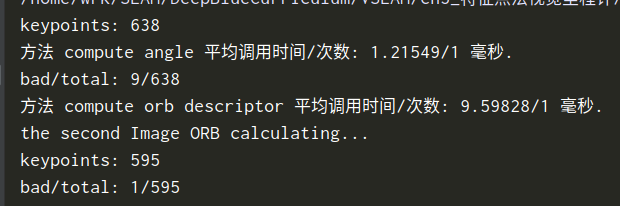
\includegraphics[width=4.8in]{ch5_2_2.png} {图2.2 描述子计算结果}
\end{figure}

\subsection{暴力匹配}
主要是调用之前计算的角度和描述子,遍历描述子1和描述子2,计算描述子不相同时的汉明距离,距离小于阈值的,取最小的作为匹配点,核心代码如Listing3,匹配结果如图2.3:(在调试过程中发现之前的描述子计算出现了错误,排查原因是自己写代码太粗心了,犯了低级错误,多套了层循环,而且计算旋转过后的p',q'的式子也没列完整,细心!!!)
\begin{lstlisting}[language=C++, caption=computeORB.cpp]
// brute-force matching
void bfMatch(const vector<DescType> &desc1, const vector<DescType> &desc2,
             vector<cv::DMatch> &matches) {
  int d_max = 50;

  // START YOUR CODE HERE (~12 lines)
  // find matches between desc1 and desc2.  核心方法是按位异或^,但是这里是按照vector<bool>的每一位来判断
    for(size_t i1=0; i1<desc1.size(); ++i1)
    {
        if(desc1[i1].empty()) continue;
        cv::DMatch m{i1, 0, 256};  //DMatch(int _queryIdx, int _trainIdx, float _distance):_queryIdx:为第i1个点进行匹配; _trainIdx:目标点匹配点为第0个;_distance:最小距离初始化为256
        for(size_t i2=0;i2<desc2.size();++i2)
        {
            if(desc2[i2].empty()) continue;
            int hanming_distance = 0;

            for(unsigned int j=0; j!=256; ++j)  //暴力匹配desc1和desc2中所有的关键点
            {
                hanming_distance += desc1[i1][j] ^ desc2[i2][j];   //不相等时距离增加
            }

            if(hanming_distance<d_max && hanming_distance<m.distance)  //如果distance符合阈值且小于现在的distance,更新最小distance和最佳匹配点
            {
                m.queryIdx = i1;        //被匹配点
                m.trainIdx = i2;        //更新最佳匹配点
                m.distance = hanming_distance;  //更新最小distance
            }
        }
        //匹配成功的
        if(m.distance<d_max)
            matches.push_back(m);
    }
  // END YOUR CODE HERE

//  for (auto &m : matches) {
//    cout << m.queryIdx << ", " << m.trainIdx << ", " << m.distance << endl;
//  }
  return;
}
\end{lstlisting}

\begin{figure}[H]
\centering
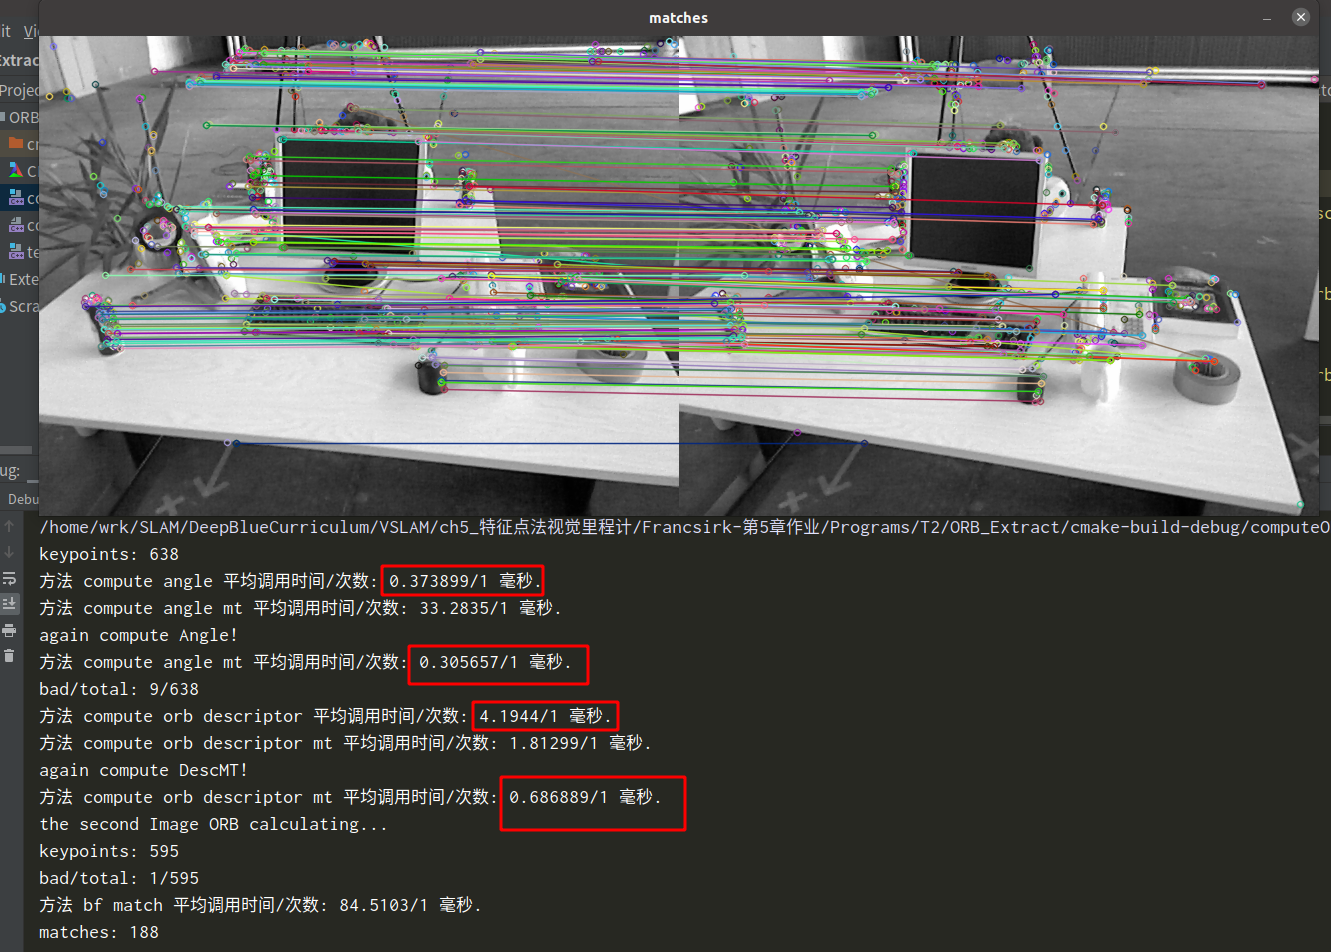
\includegraphics[width=4.8in]{ch5_2_3.png} {图2.3 匹配结果}
\end{figure}


\subsection{多线程ORB}
这部分主要按照群里助教给的文档安装了gcc,g++和tbb库,之前没安装过gcc,所以直接装上9.4版本,无需版本管理。tbb库安装时主要碰到软链接的问题,SLAM的ORB程序中需要libtbb.so.2的软链接,但是安装时只创建了libtbb.so的软链接,所以多创建一个即可。

重点是多线程程序的编写,在遍历所有特征点时,使用多线程来加速。补充一些关于多线程的知识\cite{ref2}:
\begin{figure}[H]
\centering
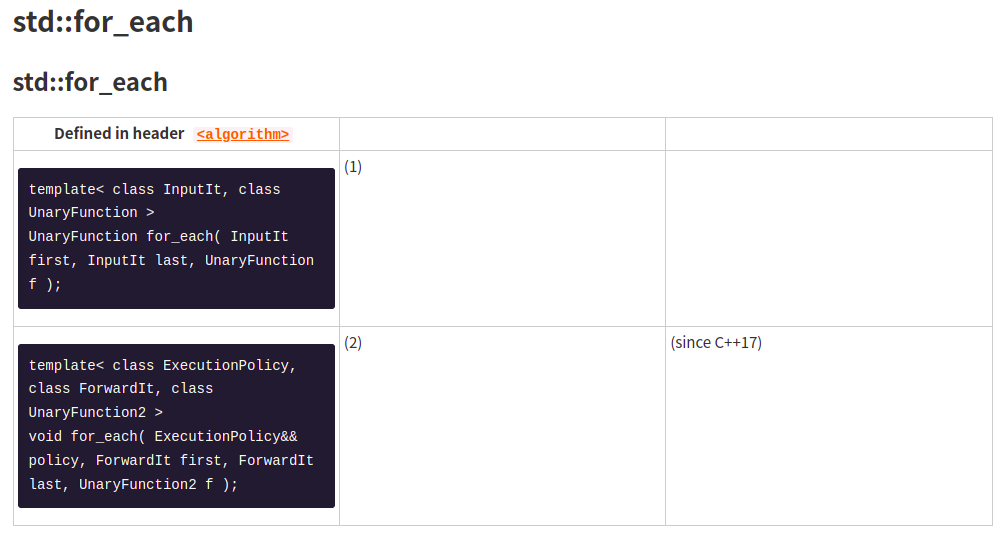
\includegraphics[width=4.8in]{ch5_2_4.png} {图2.4 std::for\_each函数}
\end{figure}

for\_each是按照迭代器来遍历元素,从C++17开始添加了执行策略ExecutionPolicy,有3种策略:
\begin{enumerate}
\item std::execution::seq  使算法在单个线程中以确定性顺序执行,即不并行且不并发;
\item std::execution::par  使算法在多个线程中执行,并且线程各自具有自己的顺序任务,即并行但不并发;
\item std::execution::par\_unseq  使算法在多个线程中执行,并且线程可以具有并发的多个任务,即并行和并发。
\end{enumerate}

first和last分别是起始和终止的迭代器,最后一个是函数f(程序里使用了lambda表达式),接受[first,last)内的迭代器。函数执行策略从C++17开始可以选择,在这里我们使用par\_unseq(并行和并发),
需要\#include <execution>。
计算Angle时不用关心数据冲突问题,因为都是使用指针进行访问,顺序无所谓,但是在计算描述子时,我们需要把计算出来的描述子push\_back到vector中,而vector是顺序容器,并行且并发不能保证push\_back的顺序,在多线程环境下,对共享的资源的插入会出现不可预知的错误。所以需要加锁保护\cite{ref3},在C++11中新增了<mutex>,我们\#include <mutex>并加锁\cite{ref4},这点至关重要,否则计算描述子只能在单线程seq中计算,最终各部分核心代码如Listing4所示,运行结果如图2.3所示。(不明白的是为什么开始计算多线程会比较慢,紧接着再调用就较快了,是否是因为有缓存?)
\begin{lstlisting}[language=C++, caption=computeORB.cpp]
void computeAngleMT(const cv::Mat &image, vector<cv::KeyPoint> &keypoints)
{
    int half_patch_size = 8;
    std::mutex m;
    //or each设计的初衷就是要遍历each one,所以只能遍历完,
    std::for_each(std::execution::par_unseq, keypoints.begin(), keypoints.end(),
                  [&half_patch_size, &image, &m](auto &kp)
                  {
                      // START YOUR CODE HERE
                      int u=kp.pt.x, v = kp.pt.y;
                      if(u>=half_patch_size && v>=half_patch_size && u+half_patch_size<=image.cols && v+half_patch_size<=image.rows)
                      {
                          float m01=0, m10=0;
                          for(int i=u-half_patch_size; i < u + half_patch_size; ++i)  //x方向遍历16个点(右)
                              for(int j=v-half_patch_size; j < v + half_patch_size; ++j)  //y方向遍历16个点(下)
                              {
                                  m10 +=i * image.at<uchar>(j, i);
                                  m01 +=j * image.at<uchar>(j, i);
                              }
                          std::lock_guard<std::mutex> guard(m);//代替m.lock; m.unlock();
                          //计算角度(弧度制)并转换为角度
                          kp.angle = (float)std::atan(m01/m10) * 180/pi ;  //或者std::atan2(m01, m10)*180/pi;
                      }
                      // END YOUR CODE HERE
                  });
    return;
}


void computeORBDescMT(const cv::Mat &image, vector<cv::KeyPoint> &keypoints, vector<DescType> &desc)
{
    // START YOUR CODE HERE (~20 lines)
    std::mutex m;
    std::for_each(std::execution::par_unseq, keypoints.begin(), keypoints.end(),
                  [&image, &desc, &m]  (auto& kp)   //lambda表达式,这个function函数接受迭代器
                  {
                      int u = kp.pt.x, v = kp.pt.y;  //迭代器要使用->来访问成员(将解引用和成员访问.结合在一起)
                      DescType d(256, false);   //256位描述子
                      //STEP1:检查是否越界
                      if(u>=8 && v>=8 && u+8<=image.cols && v+8<=image.rows)
                      {
                          //STEP2:若不越界,则根据pattern来采集点,结合特征点的方向角theta来旋转点p,q->p',q',计算p',q'的坐标,并比较大小,结果作为该位描述子的结果(0 or 1)
                          for (int i = 0; i < 256; i++)
                          {
                              // START YOUR CODE HERE (~7 lines)
                              //寻找取点pattern的下标
                              cv::Point2f p(ORB_pattern[i * 4], ORB_pattern[i * 4 + 1]);
                              cv::Point2f q(ORB_pattern[i * 4 + 2], ORB_pattern[i * 4 + 3]);

                              //使用sin,cos, 角度转换为弧度 *pi/180
                              double theta = kp.angle * pi / 180;
                              double cos_theta = cos(theta) , sin_theta = sin(theta);

                              int u_p_ = (int)(cos_theta * p.x - sin_theta * p.y) + u;
                              int v_p_ = (int)(sin_theta * p.x + cos_theta * p.y) + v;
                              int u_q_ = (int)(cos_theta * q.x - sin_theta * q.y) + u;
                              int v_q_ = (int)(sin_theta * q.x + cos_theta * q.y) + v;
                              //判断根据关键点得到的经过旋转的p、q是否出界,若出界,则该描述子清空作废
                              if(u_p_<0 || v_p_<0 || u_p_ >image.cols || v_p_ > image.rows || u_q_<0 || v_q_<0 || u_q_ >image.cols || v_q_ > image.rows)
                              {
                                  d.clear();
//                                  d = {};
                                  break;  //跳出描述子循环
                              }
                              d[i] = image.at<uchar>(v_p_, u_p_) > image.at<uchar>(v_q_, u_q_) ? false : true;  //前者大取false,后者大取true,vector随机访问器,不够快,但是掌握算法是关键
                          }
                      }
                      //越界则不使用
                      else
                      {
                          d.clear();
//                          d = {};
                      }
                      std::lock_guard<std::mutex> guard(m);//代替m.lock; m.unlock();
                      desc.push_back(d);
                  });

    int bad_points = 0;
    for(auto d:desc)
    {
        if(d.empty())
            ++bad_points;
    }
    cout << "Desc bad/total: " << bad_points << "/" << desc.size() << endl;
    return;
    // END YOUR CODE HERE
}

\end{lstlisting}

\begin{lstlisting}[language=C++, caption=CMakeLists.txt]
cmake_minimum_required(VERSION 3.21)
project(ORB_Extract)

set(CMAKE_CXX_STANDARD 17)

set(CMAKE_BUILD_TYPE "Release")
#set(CMAKE_BUILD_TYPE "Debug")
MESSAGE(STATUS "CMAKE_BUILD_TYPE IS ${CMAKE_BUILD_TYPE}")

find_package(OpenCV 3 REQUIRED)

#添加头文件
include_directories(
        ${OpenCV_INCLUDE_DIRS}
        ${G2O_INCLUDE_DIRS}
        ${Sophus_INCLUDE_DIRS}
        "/usr/local/include/eigen3/"
)

# 手写ORB特征
add_executable(computeORB computeORB.cpp)
#链接OpenCV库和tbb库
target_link_libraries(computeORB ${OpenCV_LIBS} tbb)
\end{lstlisting}


\subsection{问题回答}
\begin{enumerate}
\item 为什么说 ORB 是一种二进制特征?

因为ORB特征是使用二进制码来表示的,按照一定规则取点,比较其亮度大小,前者大则该位为0,否则为1,其实是计算若干对点亮度大小的汉明距离。
\item 为什么在匹配时使用 50 作为阈值,取更大或更小值会怎么样?

是匹配时的汉明距离的一个阈值上限,通过实验的经验而得,阈值取大会有更多误匹配点,取小会使匹配点变少。

\item 暴力匹配在你的机器上表现如何?你能想到什么减少计算量的匹配方法吗?

暴力匹配很好实现,我的机器上84ms匹配完成,速度较慢,书上提及了快速近似最近邻(FLANN)算法适用于匹配点数量极多的情况。

\item 多线程版本相比单线程版本是否有提升?在你的机器上大约能提升多少性能?

多线程版本在运行时第一次总是较慢,后面再运行时速度就较快,性能有所提升。我的机器上角度计算快了23\%,描述子计算快了83\%,还是有较大提升。
\end{enumerate}

\section{从E恢复R,t}
使用Eigen的AngleAxis构建旋转向量,转为旋转矩阵,然后对E进行SVD分解,之后分别按照流程执行,最后的输出如图3.1所示,核心代码如Listing6所示。

\begin{figure}[H]
\centering
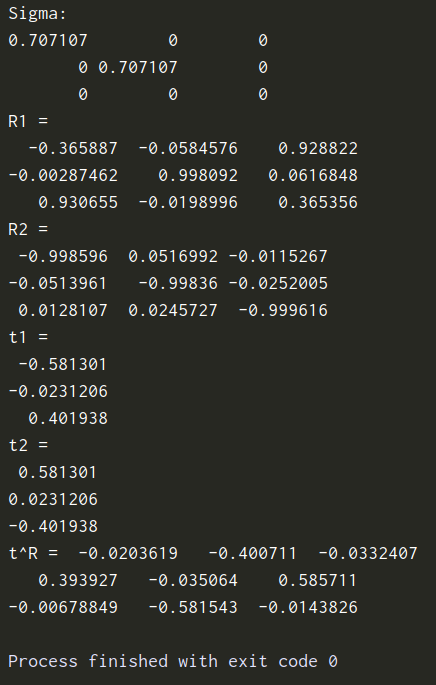
\includegraphics[scale=0.5]{ch5_3_1.png} {\\图3.1 求解的R,t结果}
\end{figure}

\begin{lstlisting}[language=C++, caption=CMakeLists.txt]
int main(int argc, char **argv) {

    // 给定Essential矩阵
    Matrix3d E;
    E << -0.0203618550523477, -0.4007110038118445, -0.03324074249824097,
            0.3939270778216369, -0.03506401846698079, 0.5857110303721015,
            -0.006788487241438284, -0.5815434272915686, -0.01438258684486258;
    // 待计算的R,t
    Matrix3d R;
    Vector3d t;
    // SVD and fix sigular values
    // START YOUR CODE HERE
    // SVD on Sigma
    Eigen::JacobiSVD<Eigen::Matrix3d> svd(E, Eigen::ComputeFullU | Eigen::ComputeFullV);  //Eigen的svd函数,计算满秩的U和V
    Eigen::Matrix3d U = svd.matrixU();
    Eigen::Matrix3d V = svd.matrixV();
    Eigen::Vector3d  sv = svd.singularValues();
    cout << "U=" << U << endl;
    cout << "V=" << V << endl;
    cout << "sv=" << sv << endl;

    Eigen::Matrix3d Sigma = Eigen::Matrix3d::Zero();
    Sigma(0,0) = sv(0);
    Sigma(1,1) = sv(1);

    cout << "Sigma:\n" << Sigma << endl;
    // END YOUR CODE HERE

    // set t1, t2, R1, R2
    // START YOUR CODE HERE

    //use AngleAxis
    Eigen::AngleAxisd rotation_vector_neg ( -M_PI/2, Eigen::Vector3d ( 0,0,1 ) );     //沿 Z 轴旋转 -90 度
    Eigen::AngleAxisd rotation_vector_pos ( M_PI/2, Eigen::Vector3d ( 0,0,1 ) );     //沿 Z 轴旋转 90 度
    Eigen::Matrix3d  RzNegHalfPi = rotation_vector_neg.toRotationMatrix();
    Eigen::Matrix3d  RzPosHalfPi = rotation_vector_pos.toRotationMatrix();


    Matrix3d t_wedge1 = U * RzPosHalfPi * Sigma * U.transpose();
    Matrix3d t_wedge2 = U * RzNegHalfPi * Sigma * U.transpose();

    Matrix3d R1 = U * RzPosHalfPi.transpose() * V.transpose();
    Matrix3d R2 = U * RzNegHalfPi.transpose() * V.transpose();
    // END YOUR CODE HERE

    cout << "R1 = \n" << R1 << endl;
    cout << "R2 = \n" << R2 << endl;
    cout << "t1 = \n" << Sophus::SO3d::vee(t_wedge1) << endl;  //求李代数??
    cout << "t2 = \n" << Sophus::SO3d::vee(t_wedge2) << endl;

    // check t^R=E up to scale
    Matrix3d tR = t_wedge1 * R1;
    cout << "t^R = " << tR << endl;

    return 0;
}
\end{lstlisting}


\section{用G-N实现Bundle Adjustment中的位姿估计}
\subsection{G-N BA}
使用高斯牛顿法进行此处的BA,要点有4个:
\begin{enumerate}
\item 数据读取 
\item 将3D数据重投影
\item 构建误差,计算雅可比(这步最难)
\item 求解方程,更新估计的位姿
\end{enumerate}
该部分核心代码如Listing7所示,结果如图4.1所示
\begin{lstlisting}[language=C++, caption=CMakeLists.txt]
int main(int argc, char **argv)
{
    VecVector2d p2d;
    VecVector3d p3d;
    Matrix3d K;
    double fx = 520.9, fy = 521.0, cx = 325.1, cy = 249.7;
    K << fx, 0, cx, 0, fy, cy, 0, 0, 1;

    // load points in to p3d and p2d
    // START YOUR CODE HERE
    double data2d[2] = {0}, data3d[3] = {0};
    ifstream fin2d(p2d_file), fin3d(p3d_file);
    for(int i=0;i<76;++i)
    {
        fin2d>>data2d[0];
        fin2d>>data2d[1];
        p2d.push_back(Eigen::Vector2d(data2d[0], data2d[1]));
        fin3d>>data3d[0];
        fin3d>>data3d[1];
        fin3d>>data3d[2];
        p3d.push_back(Eigen::Vector3d(data3d[0], data3d[1], data3d[2]));
    }

    // END YOUR CODE HERE
    assert(p3d.size() == p2d.size());

    int iterations = 100;
    double cost = 0, lastCost = 0;
    int nPoints = p3d.size();
    cout << "points: " << nPoints << endl;

    Sophus::SE3d T_esti; // estimated pose,李群,不是李代数,李代数是se3,是Vector3d

    for (int iter = 0; iter < iterations; iter++) {

        Matrix<double, 6, 6> H = Matrix<double, 6, 6>::Zero();
        Vector6d b = Vector6d::Zero();

        cost = 0;
        // compute cost  计算误差,是 观测-预测
        for (int i = 0; i < nPoints; i++)
        {
            // compute cost for p3d[I] and p2d[I]
            // START YOUR CODE HERE
        Eigen::Vector3d pc = T_esti * p3d[i];  //3D点转换到相机坐标系下(取了前3维)
        double inv_z = 1.0 / pc[2];
        double inv_z2 = inv_z * inv_z;
        Eigen::Vector2d proj(fx * pc[0] / pc[2] + cx, fy * pc[1] / pc[2] + cy);  //重投影,预测
        Eigen::Vector2d e = p2d[i] - proj;
        cost += e.transpose() * e;
	    // END YOUR CODE HERE

	    // compute jacobian
            Matrix<double, 2, 6> J;
            // START YOUR CODE HERE
        J<<fx * inv_z,
           0,
           -fx * pc[0] * inv_z2,
           -fx * pc[0] * pc[1] * inv_z2,
           fx + fx * pc[0] * pc[0] * inv_z2,
           -fx * pc[1] * inv_z,
           0,
           fy * inv_z,
           -fy * pc[1] * inv_z2,
           -fy - fy * pc[1] * pc[1] * inv_z2,
           fy * pc[0] * pc[1] * inv_z2,
           fy * pc[0] * inv_z;
        J = -J;
	    // END YOUR CODE HERE
            //高斯牛顿的系数矩阵和非齐次项
            H += J.transpose() * J;
            b += -J.transpose() * e;
        }

	// solve dx
        Vector6d dx;  //解出来的△x是李代数

        // START YOUR CODE HERE
        dx = H.ldlt().solve(b);  //解方程
        // END YOUR CODE HERE

        if (isnan(dx[0]))
        {
            cout << "result is nan!" << endl;
            break;
        }

        if (iter > 0 && cost >= lastCost) {
            // cost increase, update is not good
            cout << "cost: " << cost << ", last cost: " << lastCost << endl;
            break;
        }

        // update your estimation
        // START YOUR CODE HERE
        T_esti = Sophus::SE3d::exp(dx) * T_esti;

        // END YOUR CODE HERE

        lastCost = cost;

        cout << "iteration " << iter << " cost=" << cout.precision(12) << cost << endl;
    }

    cout << "estimated pose: \n" << T_esti.matrix() << endl;
    return 0;
}
\end{lstlisting}

\begin{figure}[H]
\centering
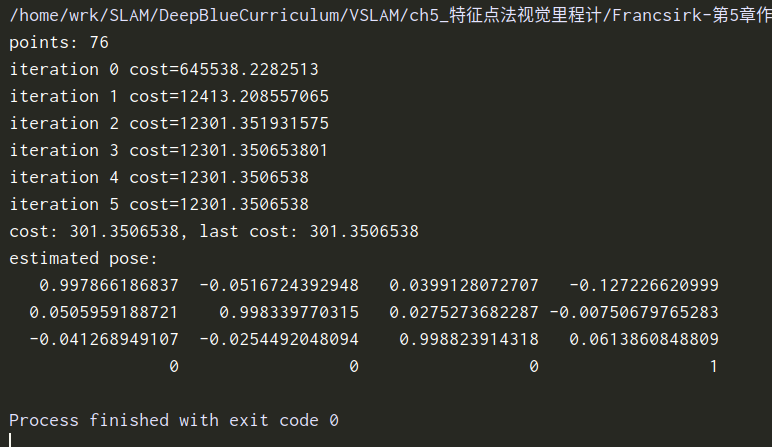
\includegraphics[scale=0.5]{ch5_4_1.png} {\\图4.1 G-N求解BA PnP结果}
\end{figure}

\subsection{问题回答}
\begin{enumerate}
\item 如何定义重投影误差?

重投影误差这里定义为观测-预测,首先将3D点通过初始化的位姿从世界系转换到相机系下,再利用相机内参和相机模型对相机下的点进行投影到归一化平面,此时就得到了预测点,再将加载出来的2d观测点与预测点的坐标作差即可得到重投影误差。

\item 该误差关于自变量的雅可比矩阵是什么?

使用李代数se(3)和李代数的左扰动模型来求解雅可比,如图4.2
\begin{figure}[H]
\centering
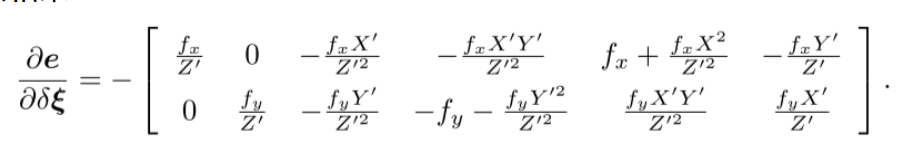
\includegraphics[scale=0.5]{ch5_4_2.png} {\\图4.2 误差关于自变量的雅可比}
\end{figure}

\item 解出更新量之后,如何更新至之前的估计上?

将dx进行指数变换成SE(3),然后左乘$pose$即可。

pose = Sophus::SE3d::exp(dx) * pose;

\end{enumerate}


\section{用ICP实现轨迹对齐}
使用第三章的轨迹绘制和读取代码进行修改,添加了手写的ICP部分的程序,最终轨迹输出如图5.1所示,$T_{ge}$的估计结果如图5.2所示,核心部分代码如Listing8所示。

思考:本身想计算出两条轨迹的RMSE,但是思考之后发现此处将平移部分看做位置P,那么两个轨迹也就相当于两帧图像,之间只有一次位姿变换T,而计算RMSE是计算整条轨迹上所有的T的误差,那么求出$T_{ge}$后对$T_e$进行变换,就能计算RMSE了。

\begin{figure}[H]
\centering
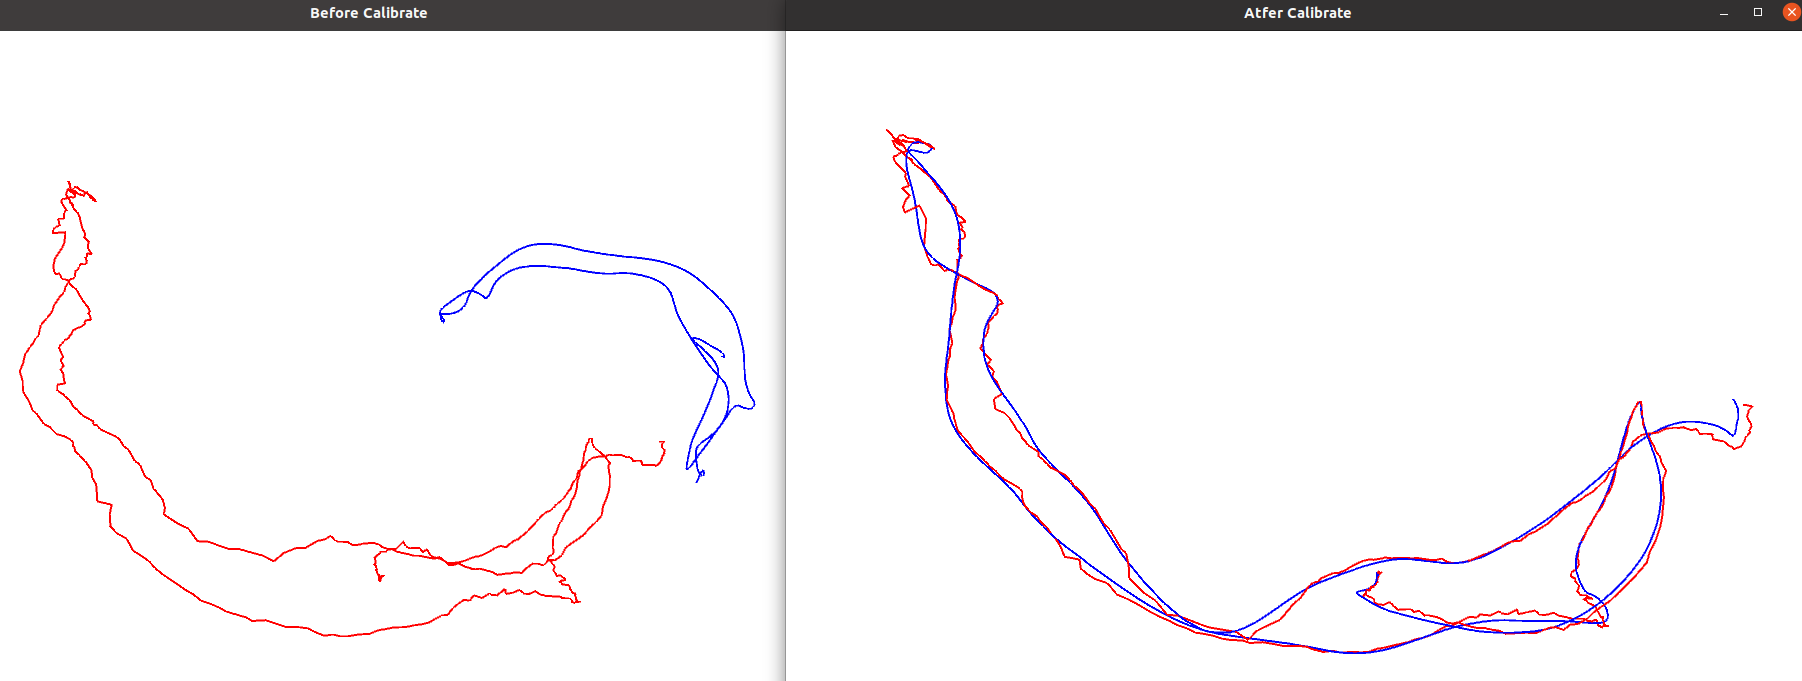
\includegraphics[scale=0.3]{ch5_5_1.png} {\\图5.1 轨迹对齐前后对比}
\end{figure}


\begin{figure}[H]
\centering
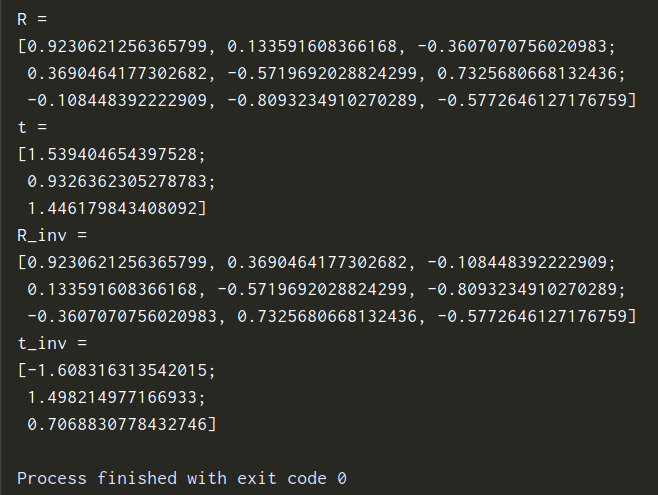
\includegraphics[scale=0.5]{ch5_5_2.png} {\\图5.2 $T_{ge}$估计结果}
\end{figure}


\begin{lstlisting}[language=C++, caption=main.cpp]
#include <iostream>
#include <fstream>
#include <unistd.h>
#include <pangolin/pangolin.h>
#include <sophus/se3.hpp>
#include <opencv2/core/core.hpp>

using namespace Sophus;
using namespace std;
using namespace cv;

string compare_file = "./compare.txt";

typedef vector<Sophus::SE3d, Eigen::aligned_allocator<Sophus::SE3d>> TrajectoryType;
typedef vector<TrajectoryType> LongTrajectoryType;
typedef Eigen::Matrix<double,6,1> Vector6d;

void DrawTrajectory(const vector<Point3d> &gt, const vector<Point3d> &esti, const string& title);
vector<TrajectoryType> ReadTrajectory(const string &path);
vector<Point3d> GetPoint(TrajectoryType TT);
void pose_estimation_3d3d(const vector<Point3d> &pts1, const vector<Point3d> &pts2, Mat &R, Mat &t);
vector<Point3d> TrajectoryTransform(Mat T, Mat t, vector<Point3d> esti );

int main(int argc, char **argv) {
    LongTrajectoryType CompareData = ReadTrajectory(compare_file);
    assert(!CompareData.empty());
    cout<<"size: "<<CompareData.size()<<endl;

    vector<Point3d> EstiPt = GetPoint(CompareData[0]);
    vector<Point3d> GtPt = GetPoint(CompareData[1]);

    Mat R, t;  //待求位姿
    pose_estimation_3d3d( GtPt, EstiPt, R, t);
    cout << "ICP via SVD results: \n" << endl;
    cout << "R = \n" << R << endl;
    cout << "t = \n" << t << endl;
    cout << "R_inv = \n" << R.t() << endl;
    cout << "t_inv = \n" << -R.t() * t << endl;

    DrawTrajectory(GtPt, EstiPt, "Before Calibrate");
    vector<Point3d> EstiCali = TrajectoryTransform(R, t, EstiPt);
    DrawTrajectory(GtPt, EstiCali, "Atfer Calibrate");
    return 0;
}

LongTrajectoryType ReadTrajectory(const string &path)
{
    ifstream fin(path);
    TrajectoryType trajectory1, trajectory2;
    if (!fin) {
        cerr << "trajectory " << path << " not found." << endl;
        return {};
    }

    while (!fin.eof()) {
        double time1, tx1, ty1, tz1, qx1, qy1, qz1, qw1;
        fin >> time1 >> tx1 >> ty1 >> tz1 >> qx1 >> qy1 >> qz1 >> qw1;
        double time2, tx2, ty2, tz2, qx2, qy2, qz2, qw2;
        fin >> time2 >> tx2 >> ty2 >> tz2 >> qx2 >> qy2 >> qz2 >> qw2;
        Sophus::SE3d p1(Eigen::Quaterniond(qw1, qx1, qy1, qz1), Eigen::Vector3d(tx1, ty1, tz1));
        trajectory1.push_back(p1);
        Sophus::SE3d p2(Eigen::Quaterniond(qw2, qx2, qy2, qz2), Eigen::Vector3d(tx2, ty2, tz2));
        trajectory2.push_back(p2);
    }
    LongTrajectoryType ret{trajectory1, trajectory2};
    return ret;
}


void DrawTrajectory(const vector<Point3d> &gt, const vector<Point3d> &esti, const string& title)
{
    // create pangolin window and plot the trajectory
    pangolin::CreateWindowAndBind(title, 1024, 768);
    glEnable(GL_DEPTH_TEST);
    glEnable(GL_BLEND);
    glBlendFunc(GL_SRC_ALPHA, GL_ONE_MINUS_SRC_ALPHA);

    pangolin::OpenGlRenderState s_cam(
            pangolin::ProjectionMatrix(1024, 768, 500, 500, 512, 389, 0.1, 1000),
            pangolin::ModelViewLookAt(0, -0.1, -1.8, 0, 0, 0, 0.0, -1.0, 0.0)
    );

    pangolin::View &d_cam = pangolin::CreateDisplay()
            .SetBounds(0.0, 1.0, pangolin::Attach::Pix(175), 1.0, -1024.0f / 768.0f)
            .SetHandler(new pangolin::Handler3D(s_cam));


    while (pangolin::ShouldQuit() == false) {
        glClear(GL_COLOR_BUFFER_BIT | GL_DEPTH_BUFFER_BIT);

        d_cam.Activate(s_cam);
        glClearColor(1.0f, 1.0f, 1.0f, 1.0f);

        glLineWidth(2);
        for (size_t i = 0; i < gt.size() - 1; i++) {
            glColor3f(0.0f, 0.0f, 1.0f);  // blue for ground truth
            glBegin(GL_LINES);
            auto p1 = gt[i], p2 = gt[i + 1];
            glVertex3d(p1.x, p1.y, p1.z);
            glVertex3d(p2.x, p2.y, p2.z);
            glEnd();
        }

        for (size_t i = 0; i < esti.size() - 1; i++) {
            glColor3f(1.0f, 0.0f, 0.0f);  // red for estimated
            glBegin(GL_LINES);
            auto p1 = esti[i], p2 = esti[i + 1];
            glVertex3d(p1.x, p1.y, p1.z);
            glVertex3d(p2.x, p2.y, p2.z);
            glEnd();
        }
        pangolin::FinishFrame();
        usleep(5000);   // sleep 5 ms
    }

}

void pose_estimation_3d3d(const vector<Point3d> &pts1,
                          const vector<Point3d> &pts2,
                          Mat &R, Mat &t) {
    Point3d p1, p2;     // center of mass 质心,这里p1表示第1幅图,p2表示第2幅图,和书上的R是反着的,所以要计算R21=这里的R12^(-1)=R12^(T),最后也输出了
    int N = pts1.size();
    for (int i = 0; i < N; i++) {
        p1 += pts1[i];
        p2 += pts2[i];
    }
    p1 = Point3d(Vec3d(p1) / N);
    p2 = Point3d(Vec3d(p2) / N);
    vector<Point3d> q1(N), q2(N); // remove the center  去质心
    for (int i = 0; i < N; i++) {
        q1[i] = pts1[i] - p1;
        q2[i] = pts2[i] - p2;
    }

    // compute q1*q2^T
    Eigen::Matrix3d W = Eigen::Matrix3d::Zero();
    for (int i = 0; i < N; i++)
    {
        W += Eigen::Vector3d(q1[i].x, q1[i].y, q1[i].z) * Eigen::Vector3d(q2[i].x, q2[i].y, q2[i].z).transpose();  //这里是2->1  R12,求R21要转置
    }
    cout << "W= \n" << W << endl;

    // SVD on W
    Eigen::JacobiSVD<Eigen::Matrix3d> svd(W, Eigen::ComputeFullU | Eigen::ComputeFullV);  //Eigen的svd函数,计算满秩的U和V
    Eigen::Matrix3d U = svd.matrixU();
    Eigen::Matrix3d V = svd.matrixV();

    cout << "U= \n" << U << endl;
    cout << "V= \n" << V << endl;

    Eigen::Matrix3d R_ = U * (V.transpose());  //这里能保证满足det(R)=1且正交吗?
    cout<<"我的输出: det(R_): "<<R_.determinant()<<"\nR_: \n"<<R_<<endl;  //Eigen的Mat
    if (R_.determinant() < 0)  //若行列式为负,取-R
    {
        R_ = -R_;
    }
    Eigen::Vector3d t_ = Eigen::Vector3d(p1.x, p1.y, p1.z) - R_ * Eigen::Vector3d(p2.x, p2.y, p2.z);   //最优的t=p-Rp'

    // convert to cv::Mat
    R = (Mat_<double>(3, 3) <<
            R_(0, 0), R_(0, 1), R_(0, 2),
            R_(1, 0), R_(1, 1), R_(1, 2),
            R_(2, 0), R_(2, 1), R_(2, 2)
    );
    t = (Mat_<double>(3, 1) << t_(0, 0), t_(1, 0), t_(2, 0));
}

vector<Point3d> GetPoint(TrajectoryType TT)
{
    vector<Point3d> pts;
    for(auto each:TT)
        //不用做相机模型的处理,也不/5000
        pts.push_back(Point3d(each.translation()[0], each.translation()[1], each.translation()[2]));
    return pts;
}

//转换
vector<Point3d> TrajectoryTransform(Mat T, Mat t, vector<Point3d> esti )
{
    vector<Point3d> calibrated={};
    Mat Mat__31;
    Sophus::SE3d SE3D;
    for(auto each:esti)
    {
        Mat__31 = (Mat_<double>(3, 1)<<each.x, each.y, each.z);
        Mat__31 = T * Mat__31 + t;
        calibrated.push_back( Point3d(Mat__31));
    }
    return calibrated;
}
\end{lstlisting}


\begin{thebibliography}{99}  
\bibitem{ref1}https://blog.csdn.net/qq\_16137569/article/details/112398976\#t5
\bibitem{ref2}https://www.w3cschool.cn/doc\_cpp/cpp-algorithm-for\_each.html?lang=en
\bibitem{ref3}https://blog.csdn.net/fengbingchun/article/details/73521630
\bibitem{ref4}https://www.cnblogs.com/thomas76/p/8554668.html
\end{thebibliography}




\end{document}